\section{Bitwise operations}
\label{sec:bitwise}
\begin{frame}<beamer>
    \frametitle{Outline}
    \tableofcontents[currentsection]
\end{frame}

\begin{frame}{What are bit operations?}
\begin{itemize}
	\item {Data onside computers are kept in binary form, such as \textcolor{blue}{10101111}}
	\vspace{0.15in}
	\item {One binary code is a data item, it could be an integer, a float number, or a string}
	\vspace{0.15in}
	\item {In some scenarios, we need to operate them bit-wisely}
\end{itemize}
	\vspace{0.25in}
\begin{itemize}
	\item {Given a binary code \textcolor{blue}{10101111}}
	\vspace{0.15in}
	\item {How could we extract out its \textcolor{red}{lower 4 bits}}
\end{itemize}
\end{frame}

\begin{frame}{The bitwise operators}
\begin{itemize}
	\item {There are \textcolor{red}{6} bit operators}
	\vspace{0.15in}
	\item {bit \textcolor{red}{and} \&}
	\vspace{0.15in}
	\item {bit \textcolor{red}{or} $|$}
	\vspace{0.15in}
	\item {bit \textcolor{red}{xor} $\hat{}$}
	\vspace{0.15in}
	\item {bit \textcolor{red}{not} $^\sim$}
	\vspace{0.15in}
	\item {\textcolor{red}{left shift} $\ll$}
	\vspace{0.15in}
	\item {\textcolor{red}{right shift} $\gg$}
\end{itemize}
\end{frame}

\begin{frame}{Truth tables for \&, $|$ and $\hat{}$}
\begin{columns}
\begin{column}{0.32\linewidth}
\begin{table}
\begin{center}
\begin{tabular}{|c|c|c|}
\hline
c1 & c2 & c1 \& c2 \\ \hline \hline
1 & 1 & 1 \\ \hline
1 & 0 & 0 \\ \hline
0 & 1 & 0 \\ \hline
0 & 0 & 0 \\ \hline
\end{tabular}
\end{center}
\end{table}
\end{column}
\begin{column}{0.32\linewidth}
\begin{table}
\begin{center}
\begin{tabular}{|c|c|c|}
\hline
c1 & c2 & c1 $|$ c2 \\ \hline \hline
1 & 1 & 1 \\ \hline
1 & 0 & 1 \\ \hline
0 & 1 & 1 \\ \hline
0 & 0 & 0 \\ \hline
\end{tabular}
\end{center}
\end{table}
\end{column}

\begin{column}{0.32\linewidth}
\begin{table}
\begin{center}
\begin{tabular}{|c|c|c|}
\hline
c1 & c2 & c1 $\hat{}$ c2 \\ \hline \hline
1 & 1 & 0 \\ \hline
1 & 0 & 1 \\ \hline
0 & 1 & 1 \\ \hline
0 & 0 & 0 \\ \hline
\end{tabular}
\end{center}
\end{table}
\end{column}
\end{columns}
\begin{itemize}
	\item {Notice that it is applied on one bit ONLY}
	\item {If there are multiple bits, the operator is applied on each bit}
	\item {The result of one bit operation has \textcolor{red}{NO} impact on the other bit}
\end{itemize}

\end{frame}

\begin{frame}[fragile]{AND $\&$ and OR $|$}
\begin{itemize}
	\item {Given two variables a = 60 and b = 13 of \textcolor{blue}{unsigned char}}
	\item {See what are the result for \textcolor{red}{a \& b}}
	\item {See what are the result for \textcolor{red}{a $|$ b}}
\end{itemize}
\begin{columns}
\begin{column}{0.5\linewidth}
\begin{figure}
\begin{center}
	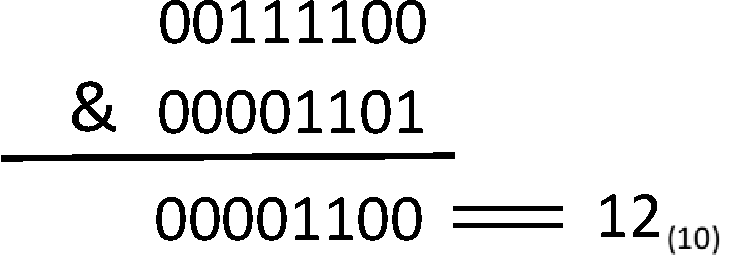
\includegraphics[width=0.8\linewidth]{figs/and.pdf}
\end{center}
\end{figure}
\end{column}
\begin{column}{0.5\linewidth}
\begin{figure}
\begin{center}
	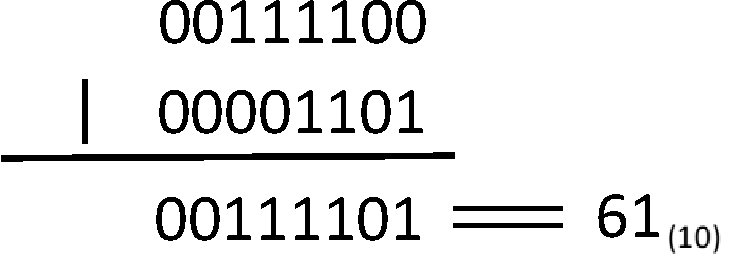
\includegraphics[width=0.8\linewidth]{figs/or.pdf}
\end{center}
\end{figure}
\end{column}
\end{columns}
\vspace{0.15in}
\begin{center}
\begin{lstlisting}[linewidth=0.7\linewidth]
#include <stdio.h>
int main(){
  unsigned char a = 60, b = 13;
  unsigned char c = a & b;
  unsigned char d = a | b;
  printf("c = %d, d = %d\n", c, d);
  return 0;
}
\end{lstlisting}
\end{center}
\end{frame}


\begin{frame}[fragile]{OR $|$ and XOR $\hat{}$}
\begin{itemize}
	\item {Given two variables a = 60 and b = 13 of \textcolor{blue}{unsigned char}}
	\item {See what are the result for \textcolor{red}{a $|$ b}}
	\item {See what are the result for \textcolor{red}{a $\hat{}$ b}}
\end{itemize}
\begin{columns}
\begin{column}{0.5\linewidth}
\begin{figure}
\begin{center}
	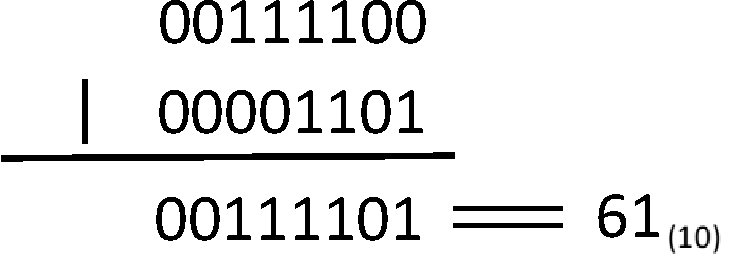
\includegraphics[width=0.8\linewidth]{figs/or.pdf}
\end{center}
\end{figure}
\end{column}
\begin{column}{0.5\linewidth}
\begin{figure}
\begin{center}
	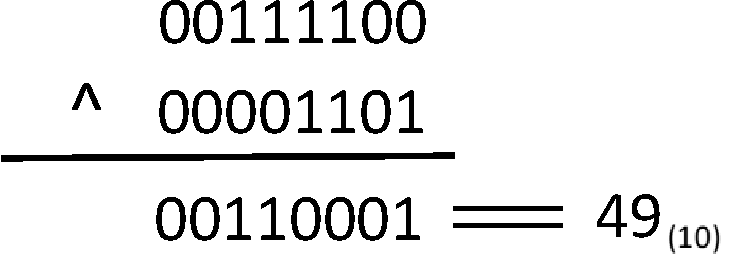
\includegraphics[width=0.8\linewidth]{figs/xor.pdf}
\end{center}
\end{figure}
\end{column}
\end{columns}
\vspace{0.15in}
\begin{center}
\begin{lstlisting}[linewidth=0.7\linewidth]
#include <stdio.h>
int main(){
  unsigned char a = 60, b = 13;
  unsigned char c = a | b;
  unsigned char d = a ^ b;
  printf("c = %d, d = %d\n", c, d);
  return 0;
}
\end{lstlisting}
\end{center}
\end{frame}


\begin{frame}[fragile]{NOT $^\sim$ (1)}
\begin{table}
\begin{center}
\begin{tabular}{|c|c|}
\hline
c1 & $^\sim$c1 \\ \hline
1 & 0  \\ \hline
0 & 1  \\ \hline
\end{tabular}
\end{center}
\end{table}
\begin{itemize}
	\item {Flip a bit}
	\item {1 $\rightarrow$ 0, 0 $\rightarrow$ 1}
	\item {The result of one bit operation has \textcolor{red}{NO} impact on the other bit}
\end{itemize}
\end{frame}

\begin{frame}[fragile]{NOT $^\sim$ (2)}
\begin{itemize}
	\item {Given one variable a = 60 of \textcolor{blue}{unsigned char}}
	\item {See what are the result for \textcolor{red}{$^\sim$a}}
\end{itemize}
\begin{figure}
\begin{center}
	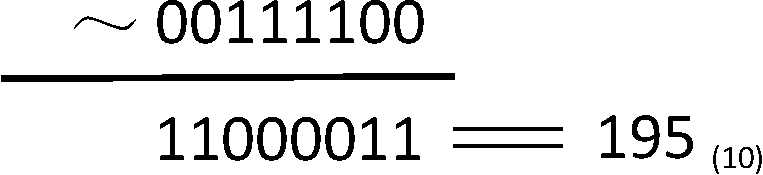
\includegraphics[width=0.4\linewidth]{figs/not.pdf}
\end{center}
\end{figure}
\vspace{0.15in}
\begin{center}
\begin{lstlisting}[linewidth=0.7\linewidth]
#include <stdio.h>
int main(){
  unsigned char a = 60;
  unsigned char c = ~a;
  unsigned char d = !a;  
  printf("c = %d, d = %d\n", c, d);
  return 0;
}
\end{lstlisting}
\end{center}
\end{frame}


\begin{frame}{Example-1: implement $\odot$ operation (1)}
\begin{table}
\begin{center}
\begin{tabular}{|c|c|c|}
\hline
c1 & c2 & c1 $\odot$ c2 \\ \hline \hline
1 & 1 & 1 \\ \hline
1 & 0 & 0 \\ \hline
0 & 1 & 0 \\ \hline
0 & 0 & 1 \\ \hline
\end{tabular}
\end{center}
\end{table}
\begin{itemize}
	\item {In some cases, we need \textcolor{red}{1} for bits of the same, while \textcolor{red}{0} for bit of difference}
	\item {There is \textcolor{red}{NO} such operator in C}
	\item {Can we realize it with provided operators?}
\end{itemize}
\begin{center}
	\Large{Think about it in five minutes...}
\end{center}

\end{frame}

\begin{frame}{Example-1: implement $\odot$ operation (2)}
\begin{figure}
\begin{center}
	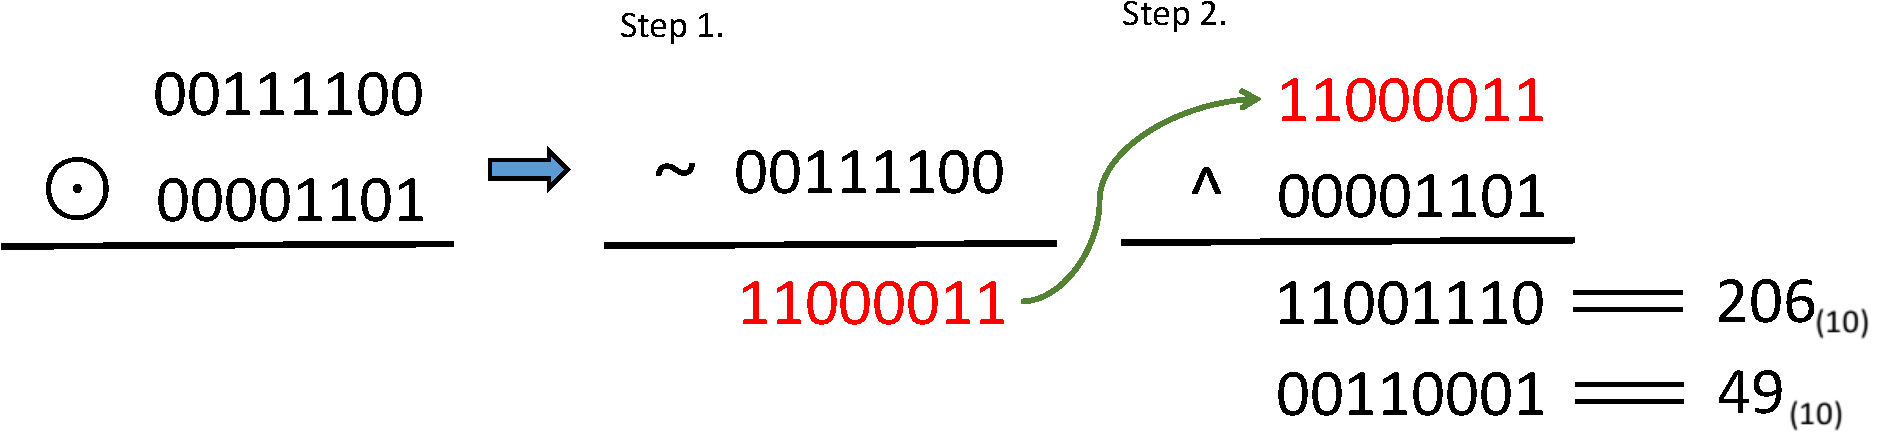
\includegraphics[width=0.95\linewidth]{figs/hor.pdf}
\end{center}
\end{figure}
\begin{itemize}
	\item {We achieve this in two steps}
	\begin{enumerate}
		\item {Flip one of the numbers}
		\item {Apply \textcolor{red}{XOR} between the flipped number and another number}
	\end{enumerate}
\end{itemize}
\end{frame}

\begin{frame}[fragile]{Example-1: implement $\odot$ operation (3)}
\vspace{-0.15in}
\begin{figure}
\begin{center}
	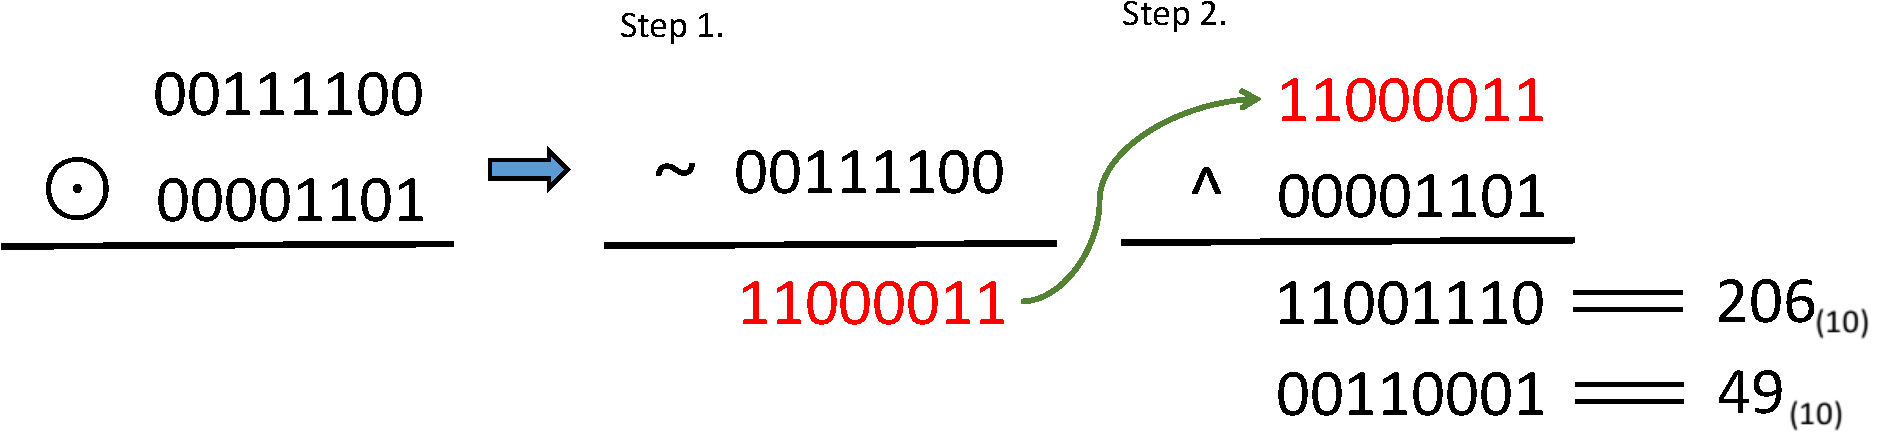
\includegraphics[width=0.95\linewidth]{figs/hor.pdf}
\end{center}
\end{figure}
\vspace{-0.15in}
\begin{lstlisting}[linewidth=0.7\linewidth]
#include <stdio.h>
int main(){
  unsigned char a = 60, b = 13;
  unsigned char c = ~a;
  unsigned char d = c ^ b;
  printf("c = %d, d = %d\n", c, d);
  return 0;
}
\end{lstlisting}
\vspace{-0.15in}
\begin{itemize}
	\item {You will get the same result if you flip b}
\end{itemize}
\end{frame}


\begin{frame}[fragile]{Left shift $val{\ll}numb$}
\vspace{-0.15in}
\begin{figure}
\begin{center}
	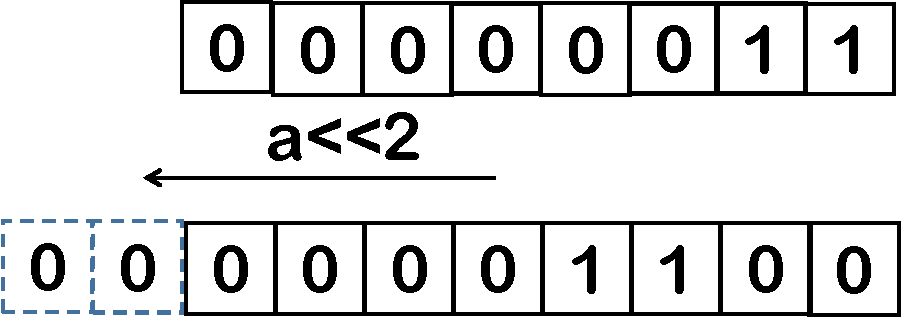
\includegraphics[width=0.5\linewidth]{figs/lshift.pdf}
\end{center}
\end{figure}
\begin{itemize}
	\item {Shift the binary code towards the left in \textcolor{red}{numb} bits}
	\item {Append the lower bits with \textcolor{red}{0}s}
	\item {For example, a = 3; \textcolor{blue}{a$\ll$2}}
	\item {The result is \textcolor{red}{12}}
\end{itemize}
\begin{lstlisting}[linewidth=0.7\linewidth]
#include <stdio.h>
int main(){
  unsigned char a = 3, b = 0;
  b = a << 2;
  printf("a = %d, b = %d\n", a, b);
  return 0;
}
\end{lstlisting}
\end{frame}


\begin{frame}[fragile]{Right shift $val{\gg}numb$}
\vspace{-0.15in}
\begin{figure}
\begin{center}
	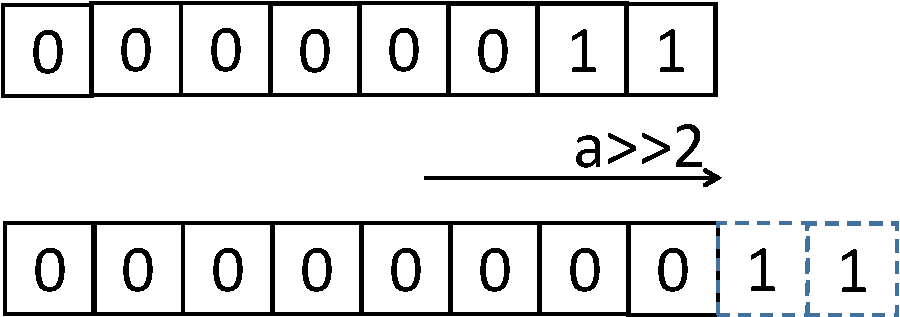
\includegraphics[width=0.5\linewidth]{figs/rshift.pdf}
\end{center}
\end{figure}
\begin{itemize}
	\item {Shift the binary code towards the right in \textcolor{red}{numb} bits}
	\item {Append the higher bits with \textcolor{red}{0}s}
	\item {For example, a = 3; \textcolor{blue}{a$\gg$2}}
	\item {The result is \textcolor{red}{0}}
\end{itemize}
\begin{lstlisting}[linewidth=0.85\linewidth]
#include <stdio.h>
int main(){
  unsigned char a = 3, b = 10, c = 0;
  b = a >> 2;
  c = a >> 1;
  printf("a = %d, b = %d, c = %d\n", a, b, c);
  return 0;
}
\end{lstlisting}
\end{frame}

\section{Applications of Bitwise operations}
\label{sec:app}
\begin{frame}<beamer>
    \frametitle{Outline}
    \tableofcontents[currentsection]
\end{frame}

\begin{frame}{Example-2: extract out specified bits from a number (1)}
\begin{itemize}
	\item {Given a binary code \textcolor{green}{10101110}}
	\vspace{0.15in}
	\item {How could we extract out its \textcolor{red}{higher 4 bits}}
	\item{Given \textcolor{blue}{int} a=\textcolor{green}{0xAE}}
\end{itemize}
\begin{center}
	\Large{Think about it in five minutes....}
\end{center}
\end{frame}

\begin{frame}{Example-2: extract out specified bits from a number (2)}
\begin{itemize}
	\item {How could we extract out its \textcolor{red}{higher 4 bits}}
	\item{Given \textcolor{blue}{int} a=\textcolor{green}{0xAE}}
	\item {We introduce a template number b = \textcolor{green}{0xF0}}
\end{itemize}
\begin{center}
	\Large{Try this operation: a \& b}
\end{center}
\end{frame}

\begin{frame}[fragile]{Example-2: extract out specified bits from a number (3)}
\begin{itemize}
	\item {How could we extract out its \textcolor{red}{higher 4 bits}}
	\item{Given \textcolor{blue}{int} a=\textcolor{green}{0xAE}}
	\item {We introduce a template number b = \textcolor{green}{0xF0}}
\end{itemize}
\begin{lstlisting}[linewidth=0.7\linewidth]
#include <stdio.h>
int main(){
  unsigned char a = 0xAE, b = 0xF0, c = 0;
  c = a & b;
  c = c>>4;
  printf("a = %x, c = %x\n", a, c);
  return 0;
}
\end{lstlisting}
\end{frame}


\begin{frame}[fragile]{Example-3: check whether  a number is odd (1)}
\begin{itemize}
	\item {Given a number \textbf{n}, we want to know whether it is odd or even}
	\item{We check \textbf{n\%2} != 1}
	\item {Now we have another option}
	\item {We only need to check the last bit of an integer number}
	\begin{enumerate}
		\item {If it is \textcolor{red}{1}, it is odd}
		\item {Otherwise, it is even}
	\end{enumerate}
\end{itemize}

\end{frame}

\begin{frame}[fragile]{Example-3: check whether  a number is odd (2)}
\begin{itemize}
	\item {Given a number \textbf{n}, we want to know whether it is odd or even}
	\item{We check \textbf{n\%2} != 1}
	\item {Now we have another option}
\end{itemize}
\begin{lstlisting}[linewidth=0.7\linewidth]
#include <stdio.h>
int main(){
  int a = 7;
  scanf("%d", &a);
  if( a & 1)
      printf("It is odd\n");
   else
      printf("It is even\n");
  return 0;
}
\end{lstlisting}
\end{frame}

\begin{frame}{Example-4: count how many bits is 1 (1)}
\begin{itemize}
	\item {Given an integer number \textbf{n}, we want to know how many bits is `1'}
	\item {We shift the number to right one bit at once}
	\item {We check whether the last bit of the shifted number is `1'}
	\begin{enumerate}
		\item {If it is \textcolor{red}{1},  counted in}
		\item {Otherwise, do nothing}
	\end{enumerate}
\end{itemize}

\end{frame}

\begin{frame}[fragile]{Example-4: count how many bits is 1 (1)}
\begin{itemize}
	\item {We shift the number to right one bit at once}
	\item {We check whether the last bit of the shifted number is `1'}
	\begin{enumerate}
		\item {If it is \textcolor{red}{1},  counted in}
		\item {Otherwise, do nothing}
	\end{enumerate}
\end{itemize}
\begin{lstlisting}[linewidth=0.7\linewidth]
#include <stdio.h>
int main(){
  int a = 11, count = 0, b = 0;
  scanf("%d", &a);
  while(a>0){
     b = a & 1;
     if(b == 1){
          count++;
     }
     a = a >> 1;
  }
  printf("count = %d\n", count);
  return 0;
}
\end{lstlisting}
\end{frame}

\begin{frame}{Example-5: set the k-th bit to 1 (1)}
\begin{itemize}
	\item {Given a number \textbf{n}=\textcolor{red}{01010000}}
	\item {We want to set the 4-th bit to \textcolor{red}{1}}
	\begin{enumerate}
		\item {We left shift \textcolor{red}{1}  3 times}
		\item {Perform OR between n and the shifted number}
	\end{enumerate}
\end{itemize}

\end{frame}

\begin{frame}[fragile]{Example-5: set the k-th bit to 1 (2)}
\begin{itemize}
	\item {Given a number \textbf{n}=\textcolor{red}{01010000}}
	\item {We want to set the 4-th bit to \textcolor{red}{1}}
	\begin{enumerate}
		\item {We left shift \textcolor{red}{1}  3 times}
		\item {Perform OR between n and the shifted number}
	\end{enumerate}
\end{itemize}
\begin{lstlisting}[linewidth=0.7\linewidth]
#include <stdio.h>
int main(){
  int a = 0x50, b = 0;
  b = 1 << 3;
  a = a | b;
  printf("count = %x\n", a);
  return 0;
}
\end{lstlisting}
\end{frame}
